\documentclass[12pt,a4paper]{article}

\usepackage[left=2cm,right=2cm,top=2cm,bottom=2cm]{geometry} % less blank area
\usepackage{amsmath,bm} % for math
\usepackage{array}   % for eqnarray
\usepackage{graphicx}
\usepackage{listings} % for code demonstration
\usepackage{color}    % for code highlight
\usepackage{fancyhdr} % for header and footnote
\usepackage{lastpage} % for calculating total pages
\usepackage{subfig} % for subfigure
\usepackage{tikz} % for drawing

\newcommand{\docTitle}{IN2106 Practical Course -- Vision-based Navigation: Exercise \#1}
\newcommand{\docAuthor}{Min-An Chao (03681062)}
\newcommand{\docAuthorDept}{TUM MS Informatics}
\newcommand{\docAuthorEmail}{ga83fok@mytum.de}
\newcommand{\docDate}{22.04.2018}

\pagestyle{fancy}
\fancyhf{}
\lhead{\textit{\docTitle}}
\rhead{\textit{\docAuthor}}
\cfoot{\textit{- Page \thepage of \pageref{LastPage} -}}

\lstset{ language={},
         basicstyle=\ttfamily\footnotesize,
         keywordstyle=\color{blue}\ttfamily\footnotesize,
         commentstyle=\color{magenta}\ttfamily\footnotesize,
         morecomment=[l][\color{magenta}\footnotesize]{\#}
}

\setlength{\parindent}{0cm}
\setlength{\parskip}{0.5cm}


\begin{document}
    \title{\vspace{-1.75cm} \large \textsf{\textbf{\docTitle}}}
    \author{\normalsize \textsf{
        \textbf{\docAuthor} \hspace{6pt}\textbar\hspace{6pt}
        \docAuthorDept \hspace{6pt}\textbar\hspace{6pt}
        \docAuthorEmail}}
    \date{\small \textsf{\docDate}}
    \maketitle 
    \thispagestyle{fancy}
    \vspace{-0.5cm}
    \hrule

    \section{What is SLAM}
   
    \textsf{\textbf{Problem 1}}
    Robots need the map to locate themselves, 
    and also the map could be used for
    providing an intuitive visualization of this environment
    for the human operator to work
    with minimized error of the robot state estimation.
    
    \textsf{\textbf{Problem 2}}
    SLAM is to provide the robot to know the map it can explore,
    and also the location it is at.
    So that further details could be added to let
    robots further know where they could move and how.

    \textsf{\textbf{Problem 3}}
    The history could be roughly divided to 2 eras,
    the classical age, from 1986 to 2004, 
    and the algorithmic analysis era, from 2004 to now.
    In the classical era,
    the main topics are probabilistic formulations for SLAM
    and the robustness and data association.
    While in algorithmic analysis era, 
    the three main topics are observability,
    convergence, and consistency.
    It is during this period,
    the main focus switched to efficient SLAM solvers
    and a lot of open source libraries are contributed.
    And recently, the rapidness of open source society
    and the low cost sensors further accelerated the
    research speed of SLAM.


    \section{Using \texttt{cmake} to manage SLAM projects written in C++}
    \textsf{\textbf{Task 1}}
    Based on the \texttt{CMakeLists.txt}
    there are 5 libraries, 
    \texttt{OpenCV}, \texttt{Pangolin}, \texttt{Eigen}, \texttt{DBoW2}, and \texttt{g2o}
    which are checked and, if not installed, then installed during \texttt{cmake}.
    After that, the main executable is compiled and built,
    then finally all the examples listed in \texttt{CMakeLists.txt}
    will be built accordingly.

    \textsf{\textbf{Task 2}}
    As shown in Fig.~\ref{fig:orbslam_snapshot},
    a video clip of my living room is fed to \texttt{ORB-SLAM2},
    meanwhile \texttt{Pangolin} is called for drawing.
    The feature points on the carpet, laptop, and stuffed toys
    could be shown marked in this snapshot.
    The estimated trajectory of the camera seems to fit its exact one.

    \begin{figure}[!h]
        \centering
        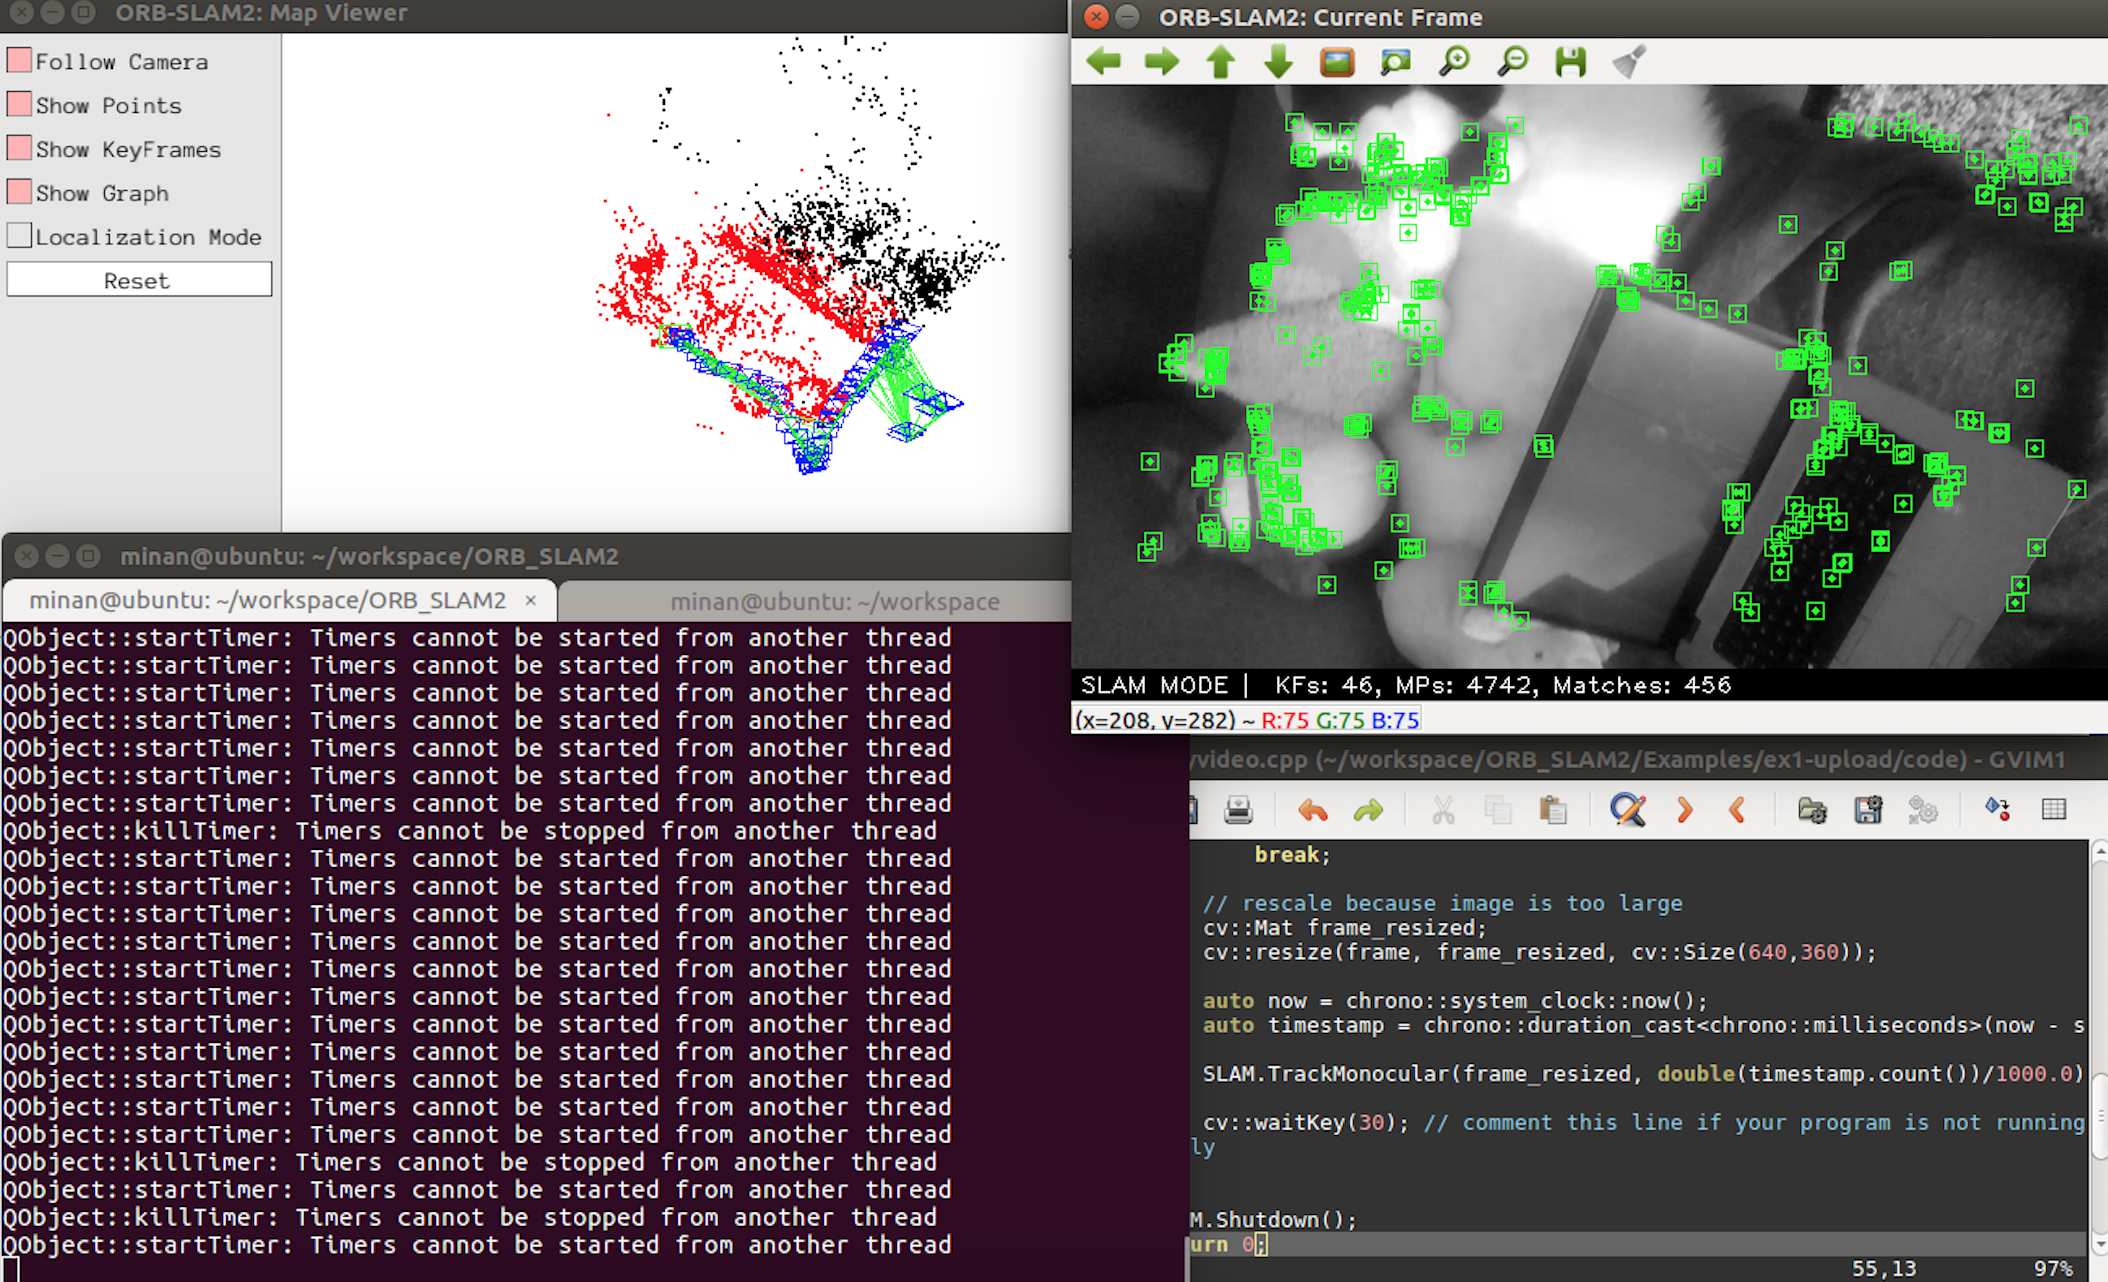
\includegraphics[height=6cm]{fig/orbslam_snapshot.png}
        \caption{Snapshot of \texttt{ORB-SLAM2} running on \texttt{mp4} video clip}
        \label{fig:orbslam_snapshot}
    \end{figure}
    
    \section{Using \texttt{Eigen} library to handle geometry computation}
    \textsf{\textbf{Task 1}}
    In this task, matrix and vector computation is used in function
    \texttt{rotation\_matrix\_rodrigues()} to do the exact Rodrigues' formula.
    The verification is done by comparing the results with 
    built-in \texttt{AngleAxisd} class. Results are shown below.
    \begin{lstlisting}[frame=single,numbers=left] 
Task 1
Given rotation vector with angle = 1.571 and rotation axis = ( 0.3333 -0.6667  0.6667)^T
Rotation matrix of Rodrigues' =
 0.1111 -0.8889 -0.4444
 0.4444  0.4444 -0.7778
 0.8889 -0.1111  0.4444
Rotation matrix from library =
 0.1111 -0.8889 -0.4444
 0.4444  0.4444 -0.7778
 0.8889 -0.1111  0.4444 
    \end{lstlisting}

    \textsf{\textbf{Task 2}}
    The dimension of imaginary part is 3, and real part 1.
    The following shows the results of 
    how quaternion multiplication is equal to matrix multiplication.
    And finally check one quaternion of its corresponding rotation matrix
    by converting between 2 representations.
    \begin{lstlisting}[frame=single,numbers=left]
Task 2
q1 = (   0.6775 -0.002796 9.851e-05    0.7355)^T
q2 = (-0.7202  0.6644  0.1312 -0.1504)^T
q1 q2     = (-0.6321  0.4001  0.5446  0.3791)^T
q1^ +  q2 = (-0.6321  0.4001  0.5446  0.3791)^T
q2^(+) q1 = (-0.6321  0.4001  0.5446  0.3791)^T
Original q = (   0.6775 -0.002796 9.851e-05    0.7355)^T
Converted rotation matrix R =
        1 -0.003933 -0.003979
-0.003643   0.08207   -0.9966
 0.004246    0.9966   0.08206
Now convert back to quaternion q' = (   0.6775 -0.002796 9.851e-05    0.7355)^T
    \end{lstlisting}

    \textsf{\textbf{Task 3}}
    By using the inversion of quaternion, 
    we can recover the world coordinates from the robot's.
    And by translating the position, and convert to another robot's
    coordinates, the answer can be carried out.
    The following shows the results.
    \begin{lstlisting}[frame=single,numbers=left]
Task 3
Object in R1's coord  = ( 0.5 -0.1  0.2)^T
Object in world coord = (-0.9958 -0.4974   0.491)^T
Object in R2's coord  = ( 1.082 0.6635  0.687)^T
    \end{lstlisting}

    
\end{document}
